
\documentclass[11pt]{report}
\usepackage{upennstyle}
\usepackage{multirow}
\usepackage[nonamebreak,round]{natbib}
\usepackage{algorithm}
\usepackage{algpseudocode}
\bibliographystyle{plainnat}
\usepackage{graphicx}
\usepackage{subcaption}
\usepackage{draftwatermark}
\usepackage{xcolor}

\SetWatermarkText{SAMPLE}
\SetWatermarkScale{3}
%\SetWatermarkColor[rgb]{1,0,0} % Red color (RGB)

%%%% TITLE PAGE
\begin{document}



\begin{mainf} % The main body of your dissertation starts below this line

\begin{Huge}
\singlespacing
    \begin{center}
    \textbf{Algorithms and Strategies for Self-Healing Chip Technology on Reconfigurable Fabric}
\end{center}
\end{Huge}



\;

\begin{center}
    Report by

    Nhlanhla Mavuso
    
\end{center} 

\;

\begin{center}
    Compiled as part of the 2023/2024 VIPER Summer Research 
\end{center}

\;

\begin{figure}[H]
    \centering
    
\includegraphics[width=0.5\linewidth]{viper_logo.png}
    \label{fig:enter-label}
\end{figure}

\begin{center}
    (Updated September 22, 2024)
\end{center}


\newpage



\textbf{Overview/Abstract}

Field Programmable Gate Arrays (FPGAs)  are susceptible to within-die process variation, aging, and environmental effects. The within-die variation accounts for a systematic, spatially-correlated, and random variation within the chip. We have demonstrated that the composite effects may account for over 190ps timing overhead on a single Look-Up Table (LUT)-to- Look-Up Table (LUT) link. Our work presents strategies and test structures to characterize the systematic variation within the chip and identify LUT-to-LUT link segments that have been exposed to the composite effects of variation and have degraded timing. We exploit online timing measurement techniques to determine the transition timing between LUT-LUT link layers on an operational circuit using a secondary clock from a Mixed Mode Clock Module (MMCM) on top of the Xilinx Artix-7 FPGA. We demonstrate that by using a Difference Detector with a Fail Latch circuit, we can estimate the delay between the LUT-LUT link layers with a resolution of  11.2ps, 14.9ps, and 17.9ps for a 1600MHz, 1200MHz, and 1000MHz Voltage-Controlled Oscillator (VCO) frequency respectively.  We also demonstrate that intra-CLB reconfiguration can fix degraded links on the fly (on an operating circuit). We have shown fixes that improve the critical path by about 10\% on a  4ns critical path running on a 100MHz clock.  Fixing the degraded links allows the chip to have more spare timing headroom that enables it to run at a lower supply voltage to minimize operational energy and/or maximize performance and throughput by increasing the operational frequency of the clock. By strategically reserving less than 5\% of chip resources and opportunistically exploiting Basic Logic Elements (BELs) and clocking resources, we achieved high-precision timing estimation (with 17.9ps resolution) and in-system intra-CLB reconfiguration in the sub-5-seconds range with pre-calculated routing tracks. 

\newpage

\section{\textbf{Introduction}}

Process variation is a major challenge in Integrated Circuit (IC) design [3]. There is uncertainty in the actual design practices, underlying process parameters, across-field effects, and environmental design characteristics[3]. The uncertainty results in die-to-die and intra-die variation. As technology nodes scale down, the effects of variation get more prominent[3]. On top of process variation, ICs are susceptible to aging, local voltage drops, local heating, and coupling effects[1]. As a result, IC Designers have employed a conservative approach to timing analysis -- accounting for worst-case temperature, voltage, and worst-case variation. However, the worst-case timing constraints are routinely greater than the silicon performance, and may sometimes be as high as 30\%[2]. For instance,  Gojman recorded sub-2ns delays to nodes predicted to have over 3ns on top of Altera Cyclone III[3]. 

However, the static-timing analysis approach employed by Gojman is offline. As technology nodes scale down, the deficiencies of static-timing analysis become even more prominent [2]. A traditional static-timing method fails to find the maximum path delays with an arbitrary covariance structure, as a result, it fails to account for circuit and input parameter variability and aging effects [2]. A probabilistic approach to static analysis may be useful, but finding bounds for a probabilistic distribution on a multivariable space is challenging. In light of these challenges, a new alternative approach to timing analysis is required -- online timing analysis. An online timing approach is implemented on a running chip and can detect the composite effects of input, circuit, location, environmental, and stochastic-depend parameters. 

Field Programmable Gates (FPGAs), unlike Application Specific Integrated Circuits (ASICs), can assign resources at a fine granularity post-fabrication. FPGAs are the best platform for investigating an online approach to timing analysis. An online approach measures the slack between two registers without disrupting an operating circuit[14]. By measuring the slack, we estimate the delay on a path. Measuring the slack also provides a diagnostic advantage to timing analysis. We use the amount of slack to determine if nodes or elements are degrading or aging, and we can also measure the composite influence of local heating, local voltage drops, environmental parameter uncertainties, and process variation. An online approach accounts for the composite effects of variation and provides a more accurate and relevant timing model. The online approach requires additional resources. It requires spare shadow registers, Programmable Interconnect Points (PIPs), LUTs, and a programmable clock. On top of the resources, it also incurs an error due to the shadow registers adding a fanout to a Basic Element of Logic (BEL) under test. There is also an error delay penalty due to the wire length from the measured BELs to the shadow registers. Previous work has shown that the effect of additional fanout is minimal (about 0.28\%) due to the pre-connected nature of an FPGA. Placing the shadow register close to the measured circuit reduces additional delay due to wire length. However, placing a shadow register increases the activity around the measured region -- which causes more local heating, local voltage drops, and coupling effects. All these need to be taken into account when determining the delay. 

We use a Difference Detector with a Fail First Fail Latch to measure LUT-to-LUT segments of an operational circuit on top of Xilinx 7-Series (Artix-7). We dynamically find a critical path and employ a basic Lateness blame calculus approach to find REG-LUT, LUT-to-LUT, or LUT-to-REG segments that have degraded (more than expected delay). Degraded segments are fixed instantaneously by finding LUT or Flip-Flop repair alternatives within the same CLB on the fly (without disruptive circuit operation).

Our Contribution include: 
\begin{enumerate}
    \item Reservation Logic
    \item On-the-Fly Delay Characterization Technique
    \item Critical Path Finder 
    \item Repair Alternative Finder 
    \item On-the-Fly CLB reconfiguration algorithm 
\end{enumerate}



\newpage

\section{\textbf{Background}}

\subsection{\textit{Process Variation}}
Lithographic variations like lens aberrations, mask errors, and variations in etch-loading are a challenge for sub-90nm technology nodes. These variations exhibit a systematic variance. As aggressive scaling continues, it also introduces non-lithographic sources of variation like well-proximity effects or dopant variation, that cause a mismatch in two identical devices or logic cells located in the same location in two dies[4].

\subsection{\textit{Local Heating, Local Voltage Drops, Local Coupling Effects}}

The delay of a measured circuit changes with the supply voltage and ambient temperature. Introducing logic adjacent to resources in a chip affects the local voltage and temperature seen by the resources. As a result,  placing logic near a circuit under measurement, whether active or not, enables a large portion of the clock networks which induces coupling effects, local voltage drops, and local heating affecting the delay of that component[5]. 

The work in this article is aware of the impact of local heating, voltage drops, and coupling effects. As a result, we demonstrate a timing model that accounts for the thermal, loading, and coupling induced by the introduction of the measurement circuit near a circuit under test, as an effort to extract a more accurate timing behavior of components or resources.  

\subsection{\textit{Aging}}

FPGA resources are expected to degrade and slow down in their lifetime.  A conservative approach to timing analysis accounts for the worst-case degradation in their expected lifetime.  This approach, however, over budgets time and energy resources, which causes severe performance and energy penalties. This means the timing and energy constraints bounds are not very tight. 

Our work is aware that the static-timing tools account for the worst-case timing aging scenarios on top of FPGAs. As a result, in our work, we also exploit the spare timing resources assigned to these resources to help increase performance and reduce overall energy consumption. 

\subsection{\textit{Dynamic Voltage and Frequency Scaling}}
With tight timing constraints, at a coarse granularity, the voltage and frequency may be adjusted to run the chip at the highest possible frequency tightly bound by the silicon performance or run the chip at a lower voltage to reduce total operational energy. 

\section{\textbf{DIFFERENCE DETECTOR WITH FIRST FAIL LATCH}}

\begin{figure}[H]
    \centering
    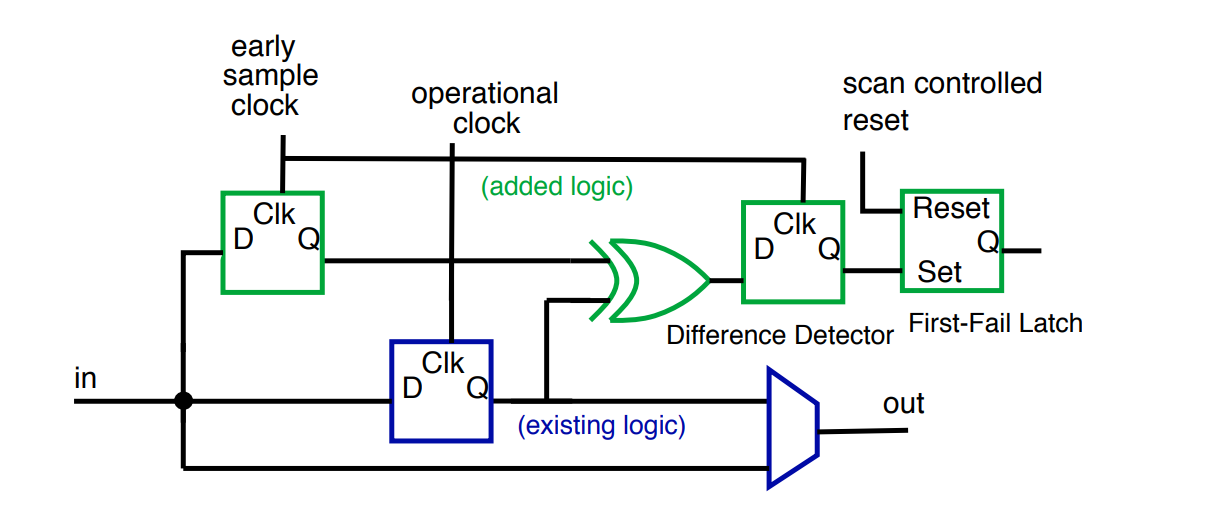
\includegraphics[width=0.55\linewidth]{ddffl.png}
    \caption{Difference Detector with First Fail Latch (adapted from COSMICTRIP)[1]}
    \label{fig:enter-label}
\end{figure}

In our work, we utilize a difference detector with a first fail latch to estimate the delay of resources on an FPGA, online. This technique utilizes a shadow register controlled by an early sample clock ($\phi_1$) that increments in small steps -- round-robin style. The number of increments is proportional to the amount of slack available on a path. The value stored by the shadow register is compared to the value stored in the circuit's operational register, and a latch is locked as soon as a difference is detected between the two registers[6]. 

\section{\textbf{LINK TIMING}}
We need to estimate the delay of the critical path of the FPGA online. From an implemented design, we convert the bit-stream to FPGA assembly where we use a host computer to find the exact locations of every single register on the design. And we find which output is the latest to arrive, this is the end of a critical path. It is possible to backtrack and find the exact wires and LUTs that are in the critical path. The critical path may not involve registers. For example, a critical path may run from an \textit{input} pin to an \textit{output} pin. Our work does not address the extreme version of the challenge. For simplicity, we require every critical path to be register terminated. 

It's not enough to find the critical path, we also need to find which LUT or hop is responsible for making the output late. We use a lateness blame approach to achieve this. We measure all the REG-to-LUT, LUT-to-LUT, or LUT-to-REG links. We assign blame to each of the links and identify which link is responsible. 


\section{\textbf{VARIATION}}

\begin{figure}[htp]
    \centering
    \begin{subfigure}[b]{0.45\textwidth}
        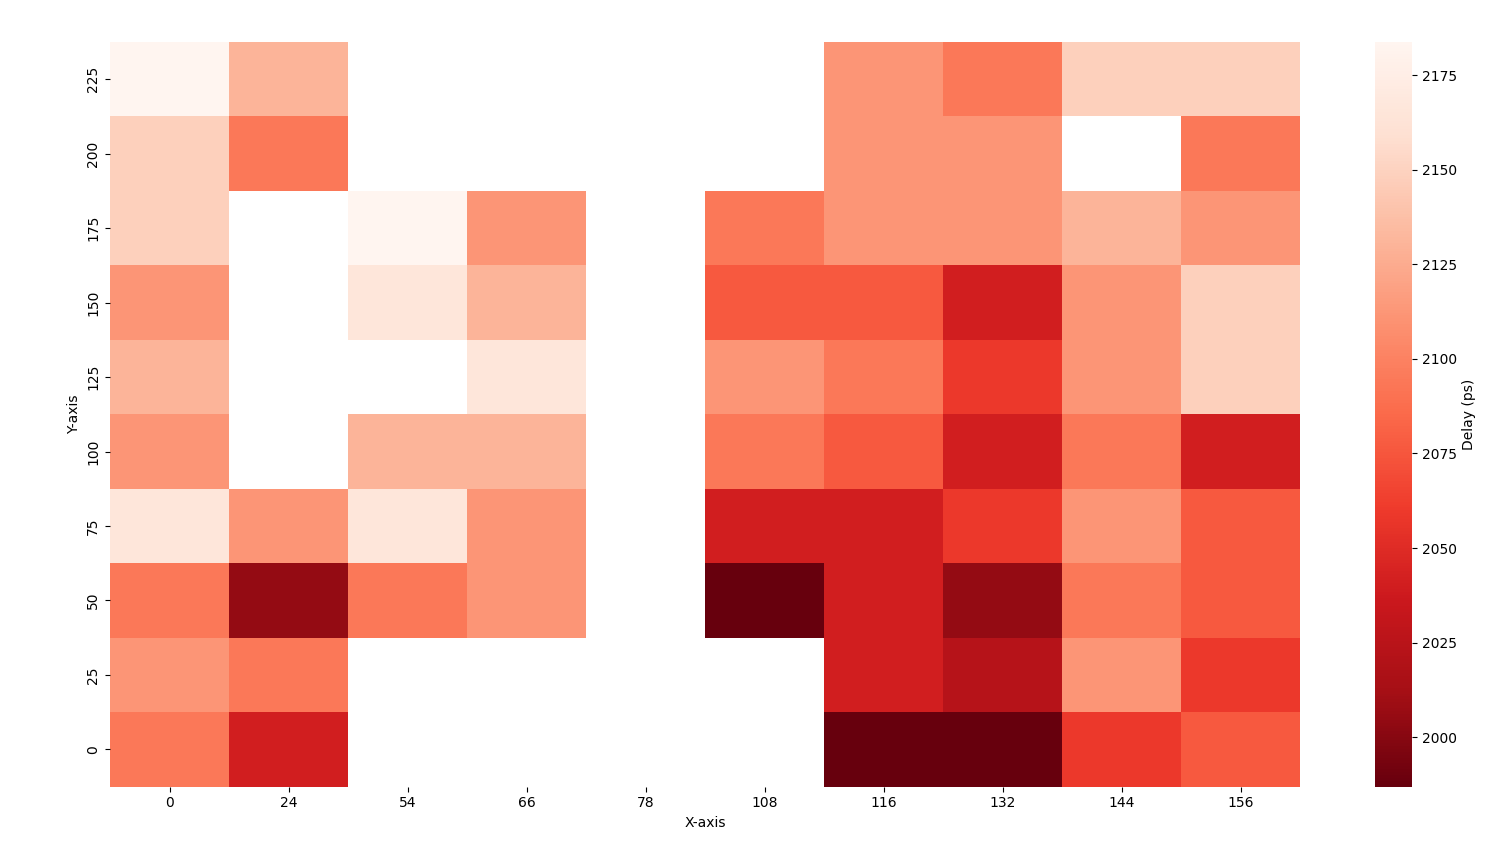
\includegraphics[width=\textwidth]{image.png}
        \caption{28nm Xilinx Artix-7 chip 1 delay mapping, showing process variation}
        \label{fig:image1}
    \end{subfigure}
    \hfill
    \begin{subfigure}[b]{0.45\textwidth}
        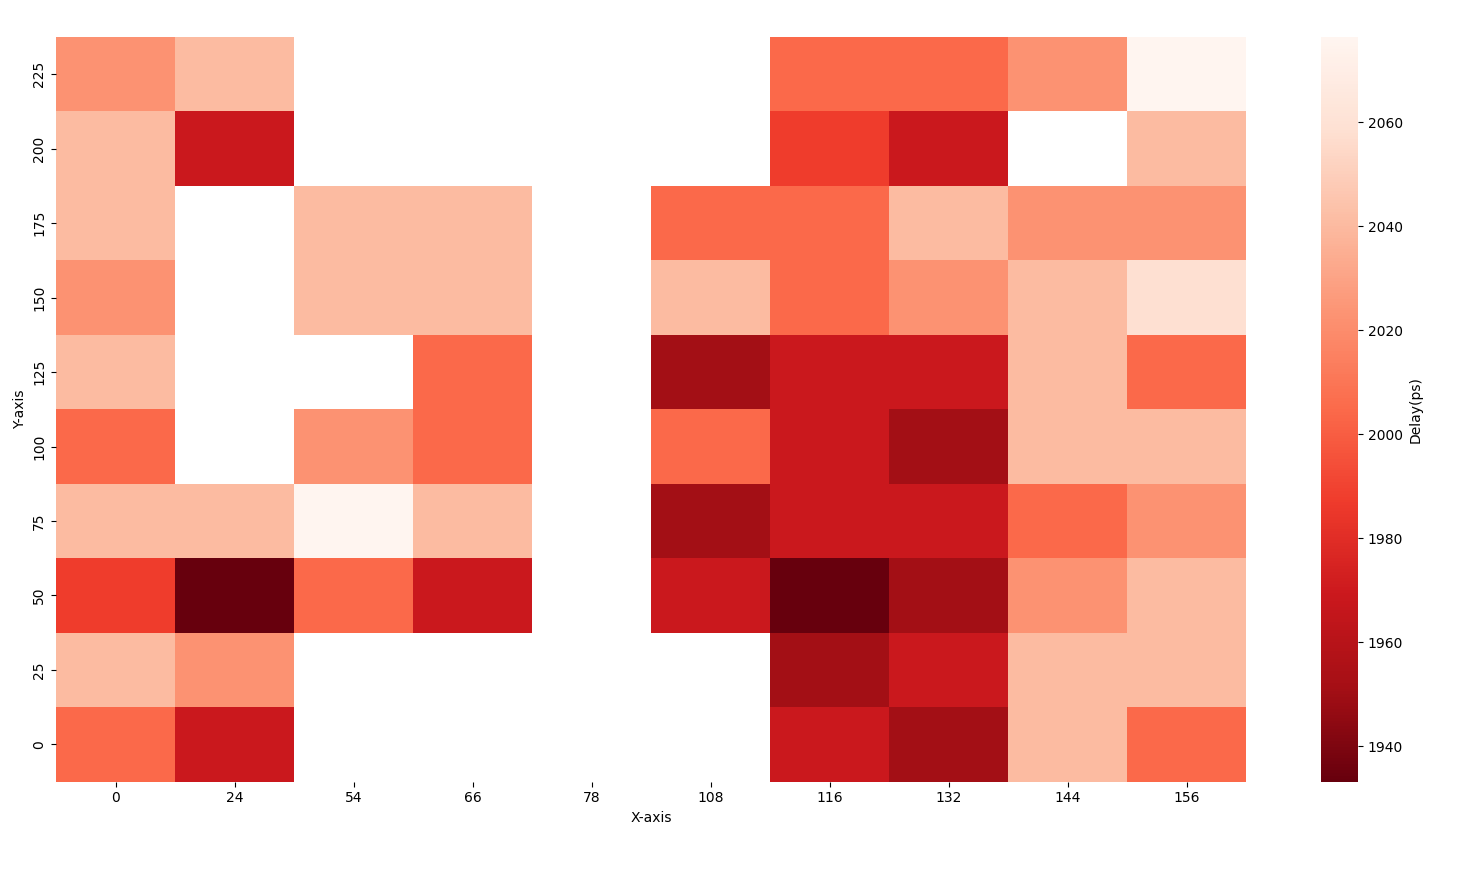
\includegraphics[width=\textwidth]{chip_2_variation.png}
        \caption{28nm Xilinx Artix-7 chip 2 delay mapping,  showing process variation.}
        \label{fig:image2}
    \end{subfigure}
\end{figure}

Figures 2a and 2b show the delay of LUT-LUT links on top of a 28nm process FPGA measured using an online measurement technique. From the heat maps, there is a clear spatial dependency of delay. Some regions, especially near the middle are much faster than the edges. Differences were measured to be as large as 190ps on a single LUT-LUT link. 

\begin{figure}[H]
    \centering
    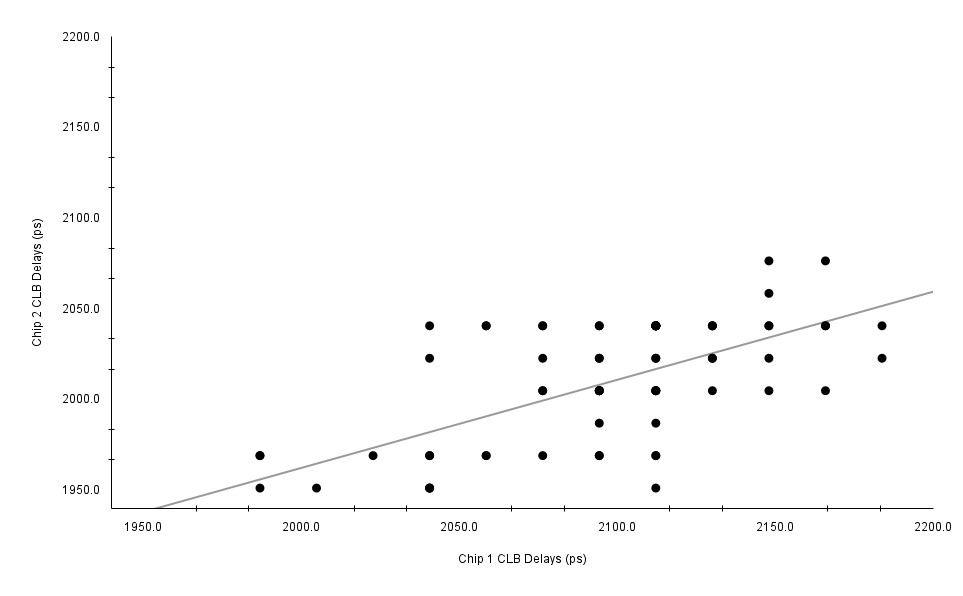
\includegraphics[width=0.5\linewidth]{correlation.png}
    \caption{Correlation between two dies, showing die-to-die variation}
    \label{fig:enter-label}
\end{figure}

Figure 3, shows the correlation of the delay from two devices (2a and 2b). The correlation graph is shifted to the right -- indicating that device 2b is slightly faster than device 2a. Die 2a had an average CLB delay of 2095.3 ps whilst die 2b had an average delay of 2008.5 ps -- making 2b 86.8ps faster on average. 


\section{\textbf{LOCAL HEATING, COUPLING, VOLTAGE DROPS}}

\begin{figure}[H]
    \centering
    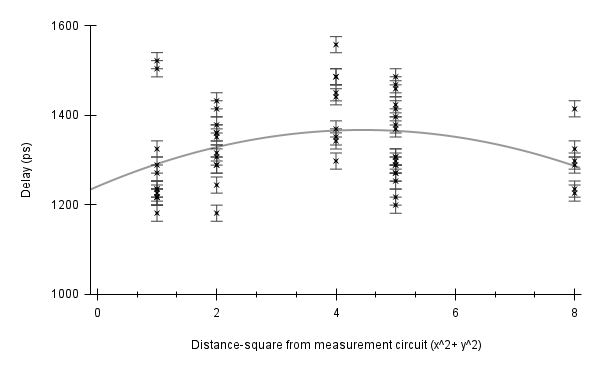
\includegraphics[width=0.5\linewidth]{distance-square.png}
    \caption{Distance-squared $(x^2 + y^2)$ from measure circuit to measured resource}
    \label{fig:enter-label}
\end{figure}


Figure 4 shows an inverted parabolic relationship between the distance of resources from a measurement circuit and the actual measured delay values (for close BELs). We expect a linear relationship once the resources are relatively far from the measurement circuit. According to Figure 4, closer resources have an overall better measurement. As the distance increases, we see an increase in the delay of the resources we measure. Initially, we thought the cause of the additional delay was the wire length. But as we keep increasing the distance, we see a decrease in the measured delay. This is striking! How can more distant resources have a lower measured delay? Resources that are too close to the measurement circuitry record less error on average because they exploit the benefit of a short wire length. As we increase the distance from the measurement circuit, the overall wire length increases. However, there is another variable -- measurement circuit activity-induced delay. The measurement circuit activates clock routing networks, causes a local voltage drop, and creates local self-heating. Closer resources are more vulnerable to these parasitic conditions. As a result, middles-distanced resources are measured to be much slower. The middle-distanced resources are at a compound vulnerability -- relatively long wire length compared to closer resources and feeling a relatively high measurement circuit activity compared to distant resources.  

\newpage

\section{\textbf{RESERVATION AND COVERAGE}} 

\begin{figure}[H]
    \centering
    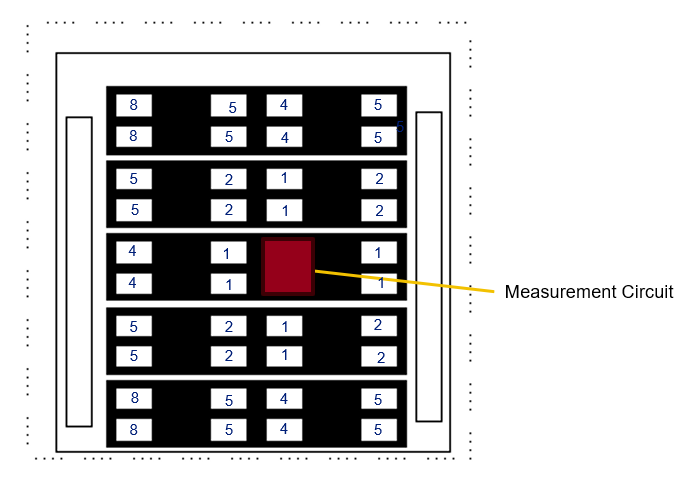
\includegraphics[width=0.5\linewidth]{clb_blocks.png}
    \caption{CLB blocks in a 4 x 5 CLB tile}
    \label{fig:enter-label}
\end{figure}


Figure 4, clearly shows that the percentage error is positional. CLBs that are too close record the lowest delay despite the influence of the measurement circuit. CLBs that are mid-distanced from the measurement circuit record the highest error due to the additive errors from wire length and measurement circuit influence. CLBs that are relatively far, away record an error that is relatively lower than middle-distanced CLBs because the largest contributing factor to the error is the wire length. The measurement circuit activity has a minimal effect on distant resources.

To minimize measurement error, we measure a resource locally, then we turn off the measurement circuit as soon as we are done making a measurement. We then measure the entire critical path with the measurement circuit on and off. From that, we determine the actual contribution of the measurement circuit to that specific resource. Another strategy is to intentionally reserve an entire CLB instead of a SLICE. We use the additional SLICE as a shield. Experiments have shown that instead of leaving the extra SLICE vacant, we can place the error capture logic there. The error capture logic is insensitive to delay. Hence, it absorbs most of the coupling effects without concern for timing. The effects of the measurement circuit activity are short-range and do not seem to have any noticeable effects beyond an interconnect tile.  


\newpage

\section{\textbf{METHOD ANALYSIS}}
 
\subsection{\textbf{FPGA Implementation}}

We use the Xilinx Artix 7 FPGA with a 28nm CMOS process with $\mu v_{th}$ of 400mV, $\sigma _{th} = 36mV$ and a typical operating $V_{dd} = 1.0V$. 

\subsection{\textbf{Experimental Architecture}}

The architecture for the FPGA consists of Configurable Logic Blocks (CLBs). In each CLB, there is a left and right SLICE. In each slice, there are four 6-Input LUTs, which each may be configured to be two 5-Input LUTs. Within the same slice, eight flip-flops can be configured as registers or latches. To support online timing measurement, we reserve an entire SLICE worth of flip-flops. We also opportunistically take advantage of unused resources (LUTs and Flip-Flops) to support the difference accumulator LUT, difference latch, Finite State Machine, and the error aggregation network. In addition, we also reserve specific tracks within a CLB to allow for intra-CLB reconfiguration.

\subsection{\textbf{Clock Generation}}

A Mixed-Mode Clock Module generates the operational clock and the early sample clock. In our case, the clocks have the same frequency of 100MHz. We fix the operational clock ($\phi_o$), and we dynamically change the phase of the early sample clock ($\phi_e)$. The size of the interpolated phase shifts depends on the Voltage-Controlled Oscillator frequency, which is directly related to the multiplicative and division factors of the early sample clock. With a VCO frequency of 1GHz, we achieve an interpolated phase shift resolution of 17.9ps. As a comparison, this resolution is 5 - 11x better than the one achieved in the Altera 65nm Cyclone III FPGA (EP3C16F484C6N)[6]. 

$$F_{vco} = F_{clkin} \times \frac{M}{D}$$

$$\alpha = \frac{1}{56 \times F_{vco}}$$

\subsection{\textbf{Experimental Procedure}}

\begin{figure}[H]
    \centering
    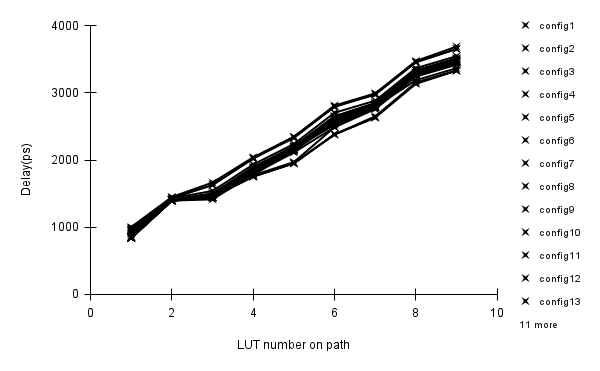
\includegraphics[width=0.5\linewidth]{path_optimization.png}
    \caption{delays on different CLB  configurations on path}
    \label{fig:enter-label}
\end{figure}
\subsubsection{Measuring the First link}

From a running circuit, we find the critical path and assign lateness blame to links. The first input-link needs to be optimal since it cannot be assigned blame. Despite its measured value, we need to exhaustively find the best LUT in the CLB it is originally located. We measure the delay of the REG-$LUT_1$ link and the total delay of the critical path using the chosen $1^{st}$ link. 

\begin{tabular}{ |p{4cm}||p{4cm}|p{4cm}|p{4cm}|  }
 \hline
 \multicolumn{4}{|c|}{Finding the best $1^{st}$ LUT for critical path} \\
 \hline
 $LUT_1$& REG-$LUT_1$ Delay (ps) &Critical Path Delay (ps)& Improvement \\
 \hline
 $CLB_L/D6LUT$   &    841.3 &3490.5& 5.34 \%\\
 $CLB_L/C6LUT $&   859.2  & 3508.4&4.87\% \\
 $CLB_L/B6LUT $ &895.0 & 3544.2&3.88\%\\
 $CLB_L/A6LUT $ &984.5& 3651.6&0.97\%\\
 $CLB_R/D6LUT $&   984.5  & 3651.6&0.97\%\\
 $CLB_R/C6LUT $& 1002.4  & 3687.4&0\% \\
 $CLB_R/B6LUT $& 859.2  & 3508.4&4.85\%\\
 $CLB_R/A6LUT $& 859.2  & 3508.4&4.85\%\\
 \hline
\end{tabular}

 Table 1. \textit{Table showing the delay of REG-$LUT_1$ links to find the best $1^{st}$ LUT. }

 

 According to Table 1, the best path should use a REG-$LUT_1$ link that involves the D6LUT in the left SLICE ($CLB_L/D6LUT$) of the original CLB location determined by VIVADO/VTR. This value is 16\% better than $CLB_R/C6LUT$. By simply using $CLB_L/D6LUT$, we are guaranteed a delay improve of 5.34\% delay improvement over the critical path that use the worst REG-$LUT_1$ link. 

 Given this insight, we greedily select the REG-$LUT_1$ link that involves $CLB_L/D6LUT$. At this point, we do not worry about the influence of the measurement circuit on the delay of the measured REG-$LUT_1$ links because we anticipate that the links experience the same measurement circuit influence and that the wire length is the same. After all, the LUTs are in the same CLB. To validate the assumption, we also measure the total critical path using the different links and compare the delay to the total critical path delay. This makes the measurement and selection of a REG-$LUT_1$ segment to be fair and judicious. 

\subsubsection{Lateness Blame}

Once we have established which REG-$LUT_1$ link is the best, we then proceed to assign lateness blame to components. 

By measuring the different delays of all the links in the critical path, link $LUT_1-LUT_2$ is assigned blame (refer to figure 6). 
\newpage
\textbf{Optimizing Latest LUT 2}

\begin{tabular}{ |p{4cm}||p{4cm}|p{4cm}|  }
 \hline
 \multicolumn{3}{|c|}{Delay of Path by changing $LUT_1 - LUT_2$ link on path} \\
 \hline
 $LUT_2$& Critical Path Delay (ps)&Improvement\\
 \hline
 $CLB_L/D6LUT $   &   3490.5
 & 5.34 \%\\
 $CLB_L/C6LUT $&   3418.9&7.28\% \\
 $CLB_L/B6LUT $ & 3472.6&5.83\%\\
 $CLB_L/A6LUT $ & 3472.6&5.83\%\\
 $CLB_R/D6LUT $&   3472.6&5.83\%\\
 $CLB_R/C6LUT $&  3418.9&7.28\% \\
 $CLB_R/B6LUT $&  3454.7&6.31\%\\
 $CLB_R/A6LUT $&  3454.7&6.31\%\\
 \hline
\end{tabular}

 Table 2. \textit{Table showing the delay of $LUT_1$-$LUT_2$ links to find the best $2^{nd}$ LUT. }

After another iteration of lateness blame, we found that the $LUT_5$ - $LUT_6$ is to be blamed as well (refer to figure 6). 

\textbf{Optimizing LUT 6}

\begin{tabular}{ |p{3cm}||p{3cm}|p{3cm}|  }
 \hline
 \multicolumn{3}{|c|}{Delay of Path by changing $6^{th}$ LUT on path} \\
 \hline
 $LUT_6$& Path Delay (ps)&Improvement\\
 \hline
 $CLB_L/D6LUT$   &  3454.7
 & 6.31 \%\\
 $CLB_L/C6LUT $&   3454.7&6.31\% \\
 $CLB_L/B6LUT $ & 3329.4&9.71\%\\
 $CLB_L/A6LUT $ &3365.2&8.74\%\\
 $CLB_R/D6LUT $&   3454.7&6.31\%\\
 $CLB_R/C6LUT $&  3472.6&5.83\% \\
 $CLB_R/B6LUT $&  3329.4&9.71\%\\
 $CLB_R/A6LUT $&  3329.4&9.71\%\\
 \hline
\end{tabular}

 Table 3. \textit{Table showing the delay of $LUT_5$-$LUT_6$ links to find the best $6^{th}$ LUT. }

By repairing $LUT_6$ we measured a nearly 10\% improvement in the delay. Therefore, the final critical path can either use the $CLB_L/B6LUT$, $CLB_R/B6LUT$, or $CLB_L/A6LUT$ for the $LUT_6$. This gives the best improvement in the overall critical path delay. 


\section{\textbf{RESULTS}}

\begin{figure}[H]
    \centering
    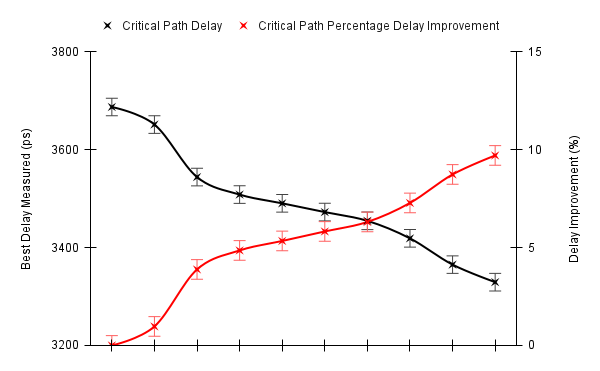
\includegraphics[width=0.75\linewidth]{delay_percent.png}
    \caption{Delay for the critical path and the critical path delay improvement}
    \label{fig:enter-label}
\end{figure}

In the example taken from a live and operating circuit, we have assigned lateness blame three times. We assigned lateness blame to REG-$LUT_1$, $LUT_1$-$LUT_2$, and $LUT_5$-$LUT_6$. This involved $27$ in different repairement options, and the best candidate was selected. Overall, we were able to achieve a delay improvement of 9.7\%. 

\section{\textbf{DISCUSSION}}
Our work promises to provide a simple and efficient way to meet tighter timing and energy constraints on technology nodes. We should be able to detect an aging LUT and find a repair alternative in the same CLB  very quickly without disrupting circuit activity. Our work is even more useful because we can meet tighter constraints amid process variation. 


\section{\textbf{FUTURE WORK}}
We are confident that our work is a step to prove the usefulness of reconfigurable computing in assigning resources at a fine granularity post-fabrication. It provide evidence that a chip that can self-heal can improve timing by about 10\%. Our work addresses problems beyond aging, including on-chip coupling effects including $v_{dd}$ drops, and local heating. This technology is implemented as a side-effect on a running chip and would be easily integrated into applications with regular downtime. There is an opportunity to heal beyond LUTs. We envision healing Digital Signal Processors (DSPs), carry chains, and Block Random Access Memories (BRAMs). On the extreme, the self-healing technology may be challenging if the healed path is healed to the point where the critical path switches -- a different path becomes the critical path. This situation is highly unlikely, but additional resources and guards need to be assigned to prevent this from happening. 

\section{\textbf{CONCLUSION}}

Online measurement investigated on FPGAs provides an efficient way to understand the distribution of variation within a running chip and helps to extrapolate an informed timing model to allow a running chip to change the placement of cells in the critical path to meet tighter timing constraints.  Without user intervention, the chip autonomously reconfigures itself to repair degrading resources. With pre-calculated routing tracks, the self-healing can be done in the sub 5-seconds. Without knowledge of the routing tracks between LUTs in the critical path, a device can repair resources in about 2 minutes -- due to a timing overheard for calculating new routing tracks. Our work has shown a self-improvement of about 10\% with reservation of only 5\% of logic resources. 

\newpage
\textbf{REFERENCES}

[1] Hans Giesen, Benjamin Gojman, Raphael Rubin, and André DeHon. 2016. Continuous online self-monitoring introspection circuitry for timing repair by incremental partial-reconfiguration (COSMIC TRIP). In Proceedings of the
FCCM. 111–118

[2] Michael Orshansky and Kurt Keutzer. 2002. A general probabilistic framework for worst-case timing analysis. In Proceedings of the 39th annual Design Automation Conference (DAC '02). Association for Computing Machinery, New York, NY, USA, 556–561. https://doi.org/10.1145/513918.514059

[3] Benjamin Gojman and André DeHon. 2014. GROK-INT: Generating real on-chip knowledge for interconnect delays
using timing extraction. In Proceedings of the IEEE Symposium on Field-Programmable Custom Computing Machines.
88–95.

[4] T. Tuan, A. Lesea, C. Kingsley and S. Trimberger, "Analysis of within-die process variation in 65nm FPGAs," 2011 12th International Symposium on Quality Electronic Design, Santa Clara, CA, USA, 2011, pp. 1-5, doi: 10.1109/ISQED.2011.5770808

[5] Timothy A. Linscott, Benjamin Gojman, Raphael Rubin, and Andre DeHon. 2016. Pitfalls and Tradeoffs in Simultaneous, On-Chip FPGA Delay Measurement. In Proceedings of the 2016 ACM/SIGDA International Symposium on Field-Programmable Gate Arrays (FPGA '16). Association for Computing Machinery, New York, NY, USA, 100–104. https://doi.org/10.1145/2847263.2847334

[6] Joshua M. Levine, Edward Stott, George A. Constantinides, and Peter Y. K. Cheung. 2012. Online Measurement of Timing in Circuits: For Health Monitoring and Dynamic Voltage \& Frequency Scaling. In Proceedings of the 2012 IEEE 20th International Symposium on Field-Programmable Custom Computing Machines (FCCM '12). IEEE Computer Society, USA, 109–116. https://doi.org/10.1109/FCCM.2012.27 

\end{mainf}    


\end{document}